\documentclass[11pt,a4paper]{article}
\usepackage{geometry}
\usepackage{changepage}
\geometry{margin=1in}
\usepackage{hyperref}
\usepackage{subcaption}
\usepackage{enumitem}
\usepackage{caption}
\usepackage{graphicx}
\title{LLM4Docq: Bootstrapping Documentation for MathComp with LLMs and Expert Feedback}
\author{
   Théo Stoskopf\thanks{Inria, CNRS, ENS de Lyon, LIP, UMR 5668, France}
  \and Jules Viennot\thanks{Inria, CNRS, Université Paris Cité, IRIF, UMR 8243, France}
  \and Cyril Cohen\footnotemark[1]
}
\date{}

\begin{document}

\maketitle

\section*{Introduction}

The \textbf{MathComp} \cite{mathcomp} library of the Rocq Prover contains thousands of definitions and lemmas, yet many currently lack detailed docstrings or explanatory comments \cite{florath2024coqlm,docstring_findings}. This scarcity of documentation creates steep learning curves for newcomers and makes it difficult to locate the right lemmas or understand formal statements \cite{Lu2025leanfinder,dvivedi2023comparative}. Recent advances in large language models (LLMs) offer a promising solution: LLMs have demonstrated an ability to generate code documentation and even assist with formal proofs in interactive theorem provers \cite{chakrabarty2024codedoc,song2025leancopilot,azerbayes2024llemma,wang2024theoremllama,kozyrev2024coqpilot}. However, directly applying general-purpose LLMs to Rocq code is non-trivial—the scarcity of training data presents unique challenges \cite{florath2024coqlm,thompson2025rango}. Addressing this gap requires \emph{domain-specific training data} and a strategy to align LLM outputs with expert knowledge \cite{ouyang2022rlhf}.

In this extended abstract, we present \textbf{LLM4Docq}, a project that aims to use LLMs and human feedback to augment MathComp with docstrings \cite{chakrabarty2024codedoc}. Our approach focuses on two key goals. First, we aim to improve \emph{user accessibility} to the MathComp library by enabling natural language retrieval of formal content \cite{Lu2025leanfinder}. Second, we fine‑tune an off-the-shelf LLM for Rocq—a model trained on Rocq code paired with docstrings—for tasks such as code auto‑completion, documentation generation, and even auto‑formalization \cite{lu2025autoformalization}. This strategy combines a \emph{user‑centric application} (search by natural language) with \emph{deep learning research} (fine‑tuning on a specialized corpus). In the following, we describe our two‑step methodology for dataset creation.

\section*{Methodology: Human‑in‑the‑Loop Documentation}

Our process consists of an \textbf{iterative human‑in‑the‑loop annotation pipeline} to efficiently bootstrap a large docstring dataset \cite{labelstudio_github}. In \textbf{Step~1}, an LLM is used to \emph{automatically generate initial docstrings} for every definition, lemma, theorem, etc., in MathComp (over 30,000 items) \cite{chakrabarty2024codedoc}. While modern models can produce plausible documentation, outputs vary in quality—some descriptions are accurate, others may be incomplete or even incorrect \cite{dvivedi2023comparative}. Rather than fully trusting these generations, we plan to incorporate \emph{expert review} to refine them \cite{ouyang2022rlhf}.

In \textbf{Step~2}, human experts will \emph{review and provide feedback} on a subset of the LLM-generated docstrings. Using a collaborative annotation platform \cite{labelstudio_github}, each candidate docstring is labeled as \textbf{Acceptable}, \textbf{Needs Improvement}, or \textbf{Incorrect}, along with corrections or suggestions when applicable (See Figure~\ref{fig:llm-examples} for examples of LLM-generated docstrings, illustrating both a typical failure and a success case as displayed in the collaborative annotation platform.). Instead of doing a full audit of the dataset, we leverage feedback from partial auditing to \emph{regenerate or improve} the remaining docstrings. For any entries annotated as "Needs Improvement" or "Incorrect" corresponding to some systemic issue, we will update the LLM prompts with additional instructions or examples derived from the expert suggestions, and have the LLM produce new versions. This targeted re‑generation uses the \emph{latest feedback as guidance}, allowing the LLM to avoid past mistakes and align with human‑preferred style and accuracy \cite{ouyang2022rlhf}. We plan to iterate this process to progressively converge on a high‑quality documentation corpus with minimal human effort on each round.

Our human‑in‑the‑loop approach is inspired by alignment techniques like reinforcement learning from human feedback, where models learn from preference data to better satisfy user intent \cite{ouyang2022rlhf}. However, instead of learning a reward model, we apply feedback \emph{directly as constraints and examples} for the next generation cycle. By leveraging LLM suggestions as a starting point and expert knowledge for correction, we expect to rapidly produce a comprehensive set of docstrings that would have otherwise required more time to author manually \cite{dvivedi2023comparative}.

\begin{figure}[h]
  \centering
  \begin{subfigure}[t]{0.45\textwidth}
    \centering
    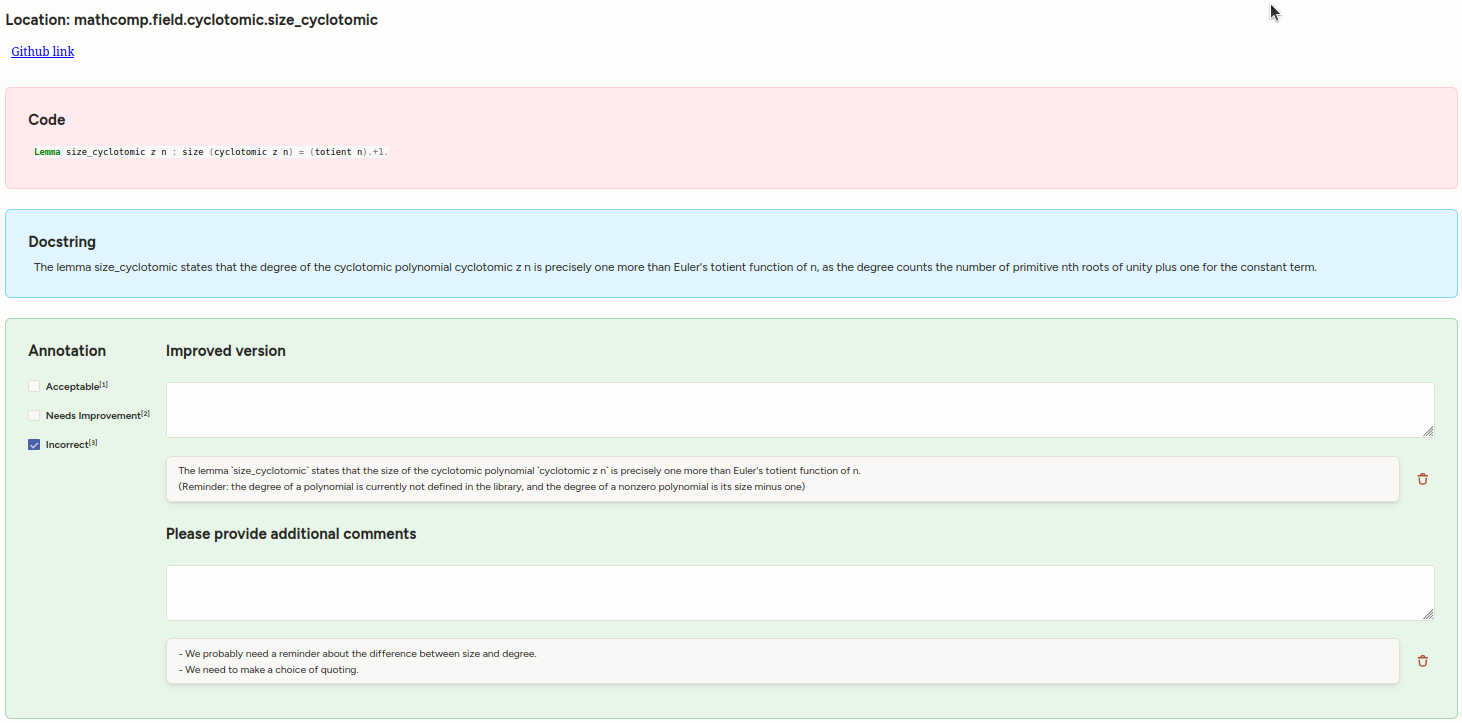
\includegraphics[width=\linewidth]{fail.png}
    \caption{Failure case}
    \label{fig:fail-case}
  \end{subfigure}%
  \hfill
  \begin{subfigure}[t]{0.45\textwidth}
    \centering
    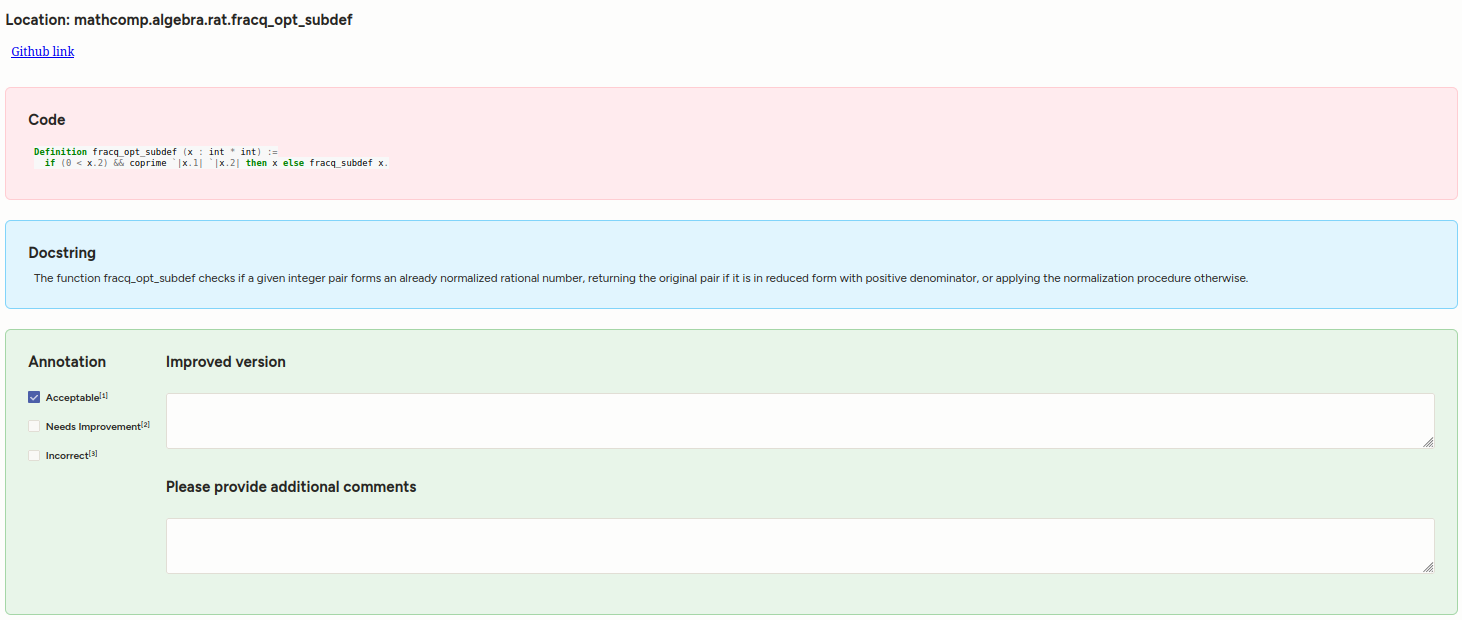
\includegraphics[width=\linewidth]{success.png}
    \caption{Success case}
    \label{fig:success-case}
  \end{subfigure}
  \caption{Illustration of LLM-generated docstrings: (a) a failure case and (b) a success case. Both cases are shown as they appear on the collaborative annotation platform.}
  \label{fig:llm-examples}
\end{figure}

\section*{LLM Fine‑Tuning on MathComp augmented with Docstrings}

The curated dataset of MathComp code annotated with reviewed docstrings enables us to train a \textbf{domain‑specific LLM} for Rocq \cite{florath2024coqlm,chakrabarty2024codedoc}. We are fine‑tuning a code‑oriented model (Qwen 2.5 32b coder base \cite{qwen25coder}) on our augmented codebase, effectively performing continued pre‑training on Rocq's formal language enriched with natural language explanations \cite{azerbayes2024llemma, wang2024theoremllama,song2025leancopilot}. This technique—\emph{training on source code together with documentation}—has precedent in software engineering: fine‑tuning an LLM on code‑comment pairs can greatly improve its ability to generate docstrings and understand code intent \cite{docstring_findings}. In our case, the model is encouraged to associate Rocq definitions/lemmas with their natural‑language descriptions \cite{azerbayes2024llemma, wang2024theoremllama}.

Recent work has combined fine-tuned LLMs on large Rocq corpora, such as CoqStoq, with retrieval-augmented generation for automatic proof synthesis \cite{thompson2025rango}. While Rango focuses on proof generation, it validates the strategy of domain‑specific fine‑tuning on formal code. Other systems, such as \emph{RocqStar}, also aim to improve the proof search in Rocq using augmented retrieval techniques \cite{kozyrev2025rocqstar}.

We plan to evaluate the final model on two complementary tasks: \begin{itemize}[leftmargin=1.5em] \item \textbf{Docstring Generation (Formal $\rightarrow$ NL):} Given a formal MathComp statement and a source code context, the model must generate an explanatory docstring \cite{chakrabarty2024codedoc}. \item \textbf{Statement Reconstruction (NL $\rightarrow$ Formal):} Given a docstring and source code context, the model must produce the corresponding Rocq formal statement (definition or lemma). This is a form of \emph{auto‑formalization} on a small scale \cite{lu2025autoformalization}. \end{itemize}

\section*{Acknowledgments}

This work has received funding from the Inria "Défi LLM4Code”. We also thank Guillaume Baudart and Marc Lelarge for their valuable input.


\bibliographystyle{plain}
\begin{thebibliography}{9}

    \bibitem{mathcomp}
    Mathematical Components Team. Mathematical Components library.
    https://github.com/math-comp/math-comp, 2007.
    
    \bibitem{song2025leancopilot}
    Peiyang Song, Kaiyu Yang, Anima Anandkumar,
    ``Towards Large Language Models as Copilots for Theorem Proving in Lean''
    \emph{arXiv preprint} 2404.12534, (2025).

    \bibitem{Lu2025leanfinder}
    Jialin Lu, Kye Emond, Weiran Sun, Wuyang Chen,
    ``Lean Finder: Semantic Search for Mathlib That Understands User Intents.''
    \emph{AI4Math Workshop @ ICML 2025}.

    \bibitem{florath2024coqlm}
    Andreas Florath,
    ``Enhancing Formal Theorem Proving: A Comprehensive Dataset for Training AI Models on Coq Code.''
    \emph{arXiv preprint} 2403.12627, (2024).

    \bibitem{qwen25coder}
    Binyuan Hui, Jian Yang, Zeyu Cui, Jiaxi Yang, Dayiheng Liu, Lei Zhang, Tianyu Liu, Jiajun Zhang, Bowen
Yu, Keming Lu, et al. Qwen2.5-Coder technical report.
    \emph{arXiv preprint} 2409.12186, (2024).

    \bibitem{ouyang2022rlhf}
    Long Ouyang , Jeff Wu, Xu Jiang, Diogo Almeida, Carroll L. Wainwright, Pamela Mishkin, Chong Zhang, Sandhini Agarwal, Katarina Slama, Alex Ray, John Schulman, Jacob Hilton, Fraser Kelton, Luke Miller, Maddie Simens, Amanda Askell, Peter Welinder, Paul Christiano, Jan Leike, Ryan Lowe
    ``Training language models to follow instructions with human feedback.''
    \emph{NeurIPS 2022}.

    \bibitem{azerbayes2024llemma}
    Zhangir Azerbayev, Hailey Schoelkopf, Keiran Paster, Marco Dos Santos, Stephen McAleer, Albert Q. Jiang, Jia Deng, Stella Biderman, Sean Welleck.
    ``Llemma: An Open Language Model For Mathematics.''
    \emph{ICLR 2024}.
    
    \bibitem{wang2024theoremllama}
    Ruida Wang, Jipeng Zhang, Yizhen Jia, Rui Pan, Shizhe Diao, Renjie Pi, Tong Zhang,
    ``TheoremLlama: Transforming General-Purpose LLMs into Lean4 Experts.''
    \emph{arXiv preprint} 2407.03203, (2024).

    \bibitem{kozyrev2024coqpilot}
    Andrei Kozyrev, Gleb Solovev, Nikita Khramov, Anton Podkopaev,
    ``CoqPilot: a plugin for LLM-based generation of proofs.''
    \emph{AITP 2024} (poster abstract).

    \bibitem{chakrabarty2024codedoc}
    Sayak Chakrabarty, Souradip Pal,
    ``ReadmeReady: Free and Customizable Code Documentation with LLMs - A Fine-Tuning Approach''
    \emph{Journal of Open Source Software} (2025).

    \bibitem{lu2025autoformalization}
    Jianqiao Lu, Yingjia Wan, Zhengying Liu, Yinya Huang, Jing Xiong, Chengwu Liu, Jianhao Shen, Hui Jin, Jipeng Zhang, Haiming Wang, Zhicheng Yang, Jing Tang, Zhijiang Guo,
    ``Process-Driven Autoformalization in Lean 4.''.
    \emph{arXiv preprint} 2406.01940, (2024).

    \bibitem{thompson2025rango}
    Kyle Thompson, Nuno Saavedra, Pedro Carrott, Kevin Fisher, Alex Sanchez-Stern, Yuriy Brun, João F. Ferreira, Sorin Lerner, Emily First,
    ``Rango: Adaptive Retrieval-Augmented Proving for Automated Software Verification.''
    \emph{ICSE 2025}.

    \bibitem{labelstudio_github}
    Label Studio, “HumanSignal/label-studio”, GitHub, 2025.

    \bibitem{docstring_findings}
    William Macke, Michael Doyle,
    ``Testing the Effect of Code Documentation on Large Language Model Code Understanding''
    \emph{Findings-NAACL}, (2024).

    \bibitem{dvivedi2023comparative}
    Shubhang Shekhar Dvivedi, Vyshnav Vijay, Sai Leela Rahul Pujari, Shoumik Lodh, Dhruv Kumar,
    ``A Comparative Analysis of Large Language Models for Code Documentation Generation,''
    \emph{First ACM International Conference on AIware}, (2024).

    \bibitem{kozyrev2025rocqstar}
    Nikita Khramov, Andrei Kozyrev, Gleb Solovev, Anton Podkopaev,
    ``RocqStar: Leveraging Similarity-driven Retrieval and Agentic Systems for Rocq generation.''
    \emph{arXiv preprint} 2505.22846, (2025).

\end{thebibliography}

\end{document}
